\section{Units and Dimensions in Nuclear Physics}
\subsection{Length}
The order of $10^{-15}$m = 1fm (fermi/femtometer) meter. This is the distance between nucleons.

\subsection{Time Scale}
\begin{itemize}
    \item $10^{-20}$s: Unbound, in the case of nuclear reactions and decays. 
    \item $10^{-9}$/$10^{-12}$s: lifetimes of excited nuclear states through gamma decays. 
    \item Minutes/hours/millions of years: Alpha and beta decays. 
\end{itemize}

\subsection{Energy}
MeV in nuclear physics. 
\begin{equation}
    1 \text{ MeV} = 1.6 \times 10^{-13} \text{J}. 
    \end{equation}
    \begin{equation}
        1 \text{eV} = 1.6 \times 10^{-19} \text{J}
        \end{equation}

\subsection{Mass}
u = unified atomic mass unit. 1 u is defined as 1/12 of the mass of an unbound $^{12}$C atom. Mass is equivalent with energy. Therefore:
\begin{equation}
u = 931.5 \text{ MeV} / c^2 = 1.66 \times 10^{-27} \text{kg}
\end{equation}
\begin{figure}[ht!]
    \centering
    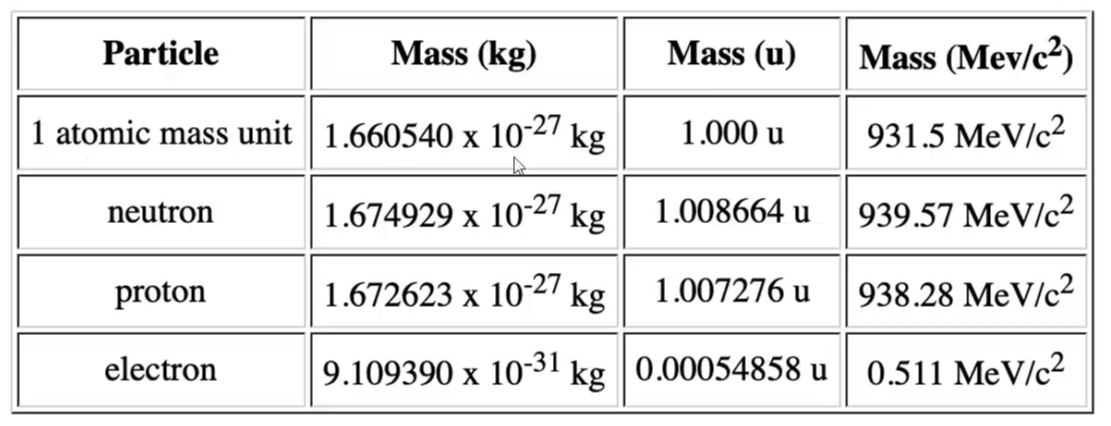
\includegraphics[width = \textwidth]{nucleon_mass_table.png}
    \caption{Table of the masses of the nucleons. $c^2 = 931.5$MeV/u. In reality, the mass of the proton is slightly less than the mass of the neutron. The proton is 2000 times more massive than the electron.}
    \label{fig: }
\end{figure}


\section{Nuclear Properties}
The parameters which describe the nucleus are. There are two types of nuclear properties: static and dynamic.
\begin{itemize}
    \item Static: Charge, Radius, mass, Binding energy, Angular momentum, Parity, Magnetic dipole moment, Electric quadrupole moments, Exited states and their energies. 
    \item Dynamic: Shape, Decay
\end{itemize}

\subsection{Connected Terms}
\begin{itemize}
    \item Charge/Charge Distribution: Protons. Found via electron scattering \cref{subsec: Nuclear Charge Distribution from Electron Scattering} by the Coulomb interaction. 
    \item Matter/Mass Distribution: Nucleons. Found via hadron scattering \cref{subsec: Nuclear Mass Distribution from Hadron Scattering}, alpha particles (Rutherford), protons and neutrons by using the strong force.
    \item Radius: Size of the nucleus (nucleons)
\end{itemize}

\subsection{Charge Distribution}
To probe the charge distribution of the nucleus, we use charged particles. We also need the following:
\begin{itemize}
    \item A beam of charged particles (often protons)
    \item Wavelength should be similar or smaller than the nucleus (about 10fm in diameter). 
    \item Electrons were popular in the 50's. 
    \item An energy of 100 Mev to 1 GeV is needed.
    \item Calculating the energy needed is done by using the de Broglie wavelength where $λ = h / p$ with $λ ≤ 10$fm. 
\end{itemize}

\subsection{Nuclear Charge Distribution from Electron Scattering}\label{subsec: Nuclear Charge Distribution from Electron Scattering}
\begin{itemize}
    \item Radius increases with mass number $A$
    \item The central nuclear charge density is nea4rly the same for all nuclei. Nucleons do not seem to concentrate near the center of the nucleus, but instead have a constant distribution along the surface. 
    \item The number of nucleons per unit volume is roughly constant:
    \begin{equation}
    \frac{A}{\frac{4}{3}πR^3} ≈ \text{const}
    \end{equation} 
    \item The radius of the nucleus is proportional to $A^{1/3}$. 
    \begin{equation}
    R = R_0A^{1/3} \quad , \quad  R_0 ≈ 1.2 \text{ fm}
    \end{equation}
\end{itemize}

\subsection{Nuclear Size}
We can find the radius of a nucleus by using the scattering angle of the local minimum of the Rutherford cross-section, see \cref{fig: electron_scattering_angles}. The diffraction pattern is not exactly that of a circular disk, as the nucleus does not have a well-defined surface.
\begin{figure}[ht!]
\centering
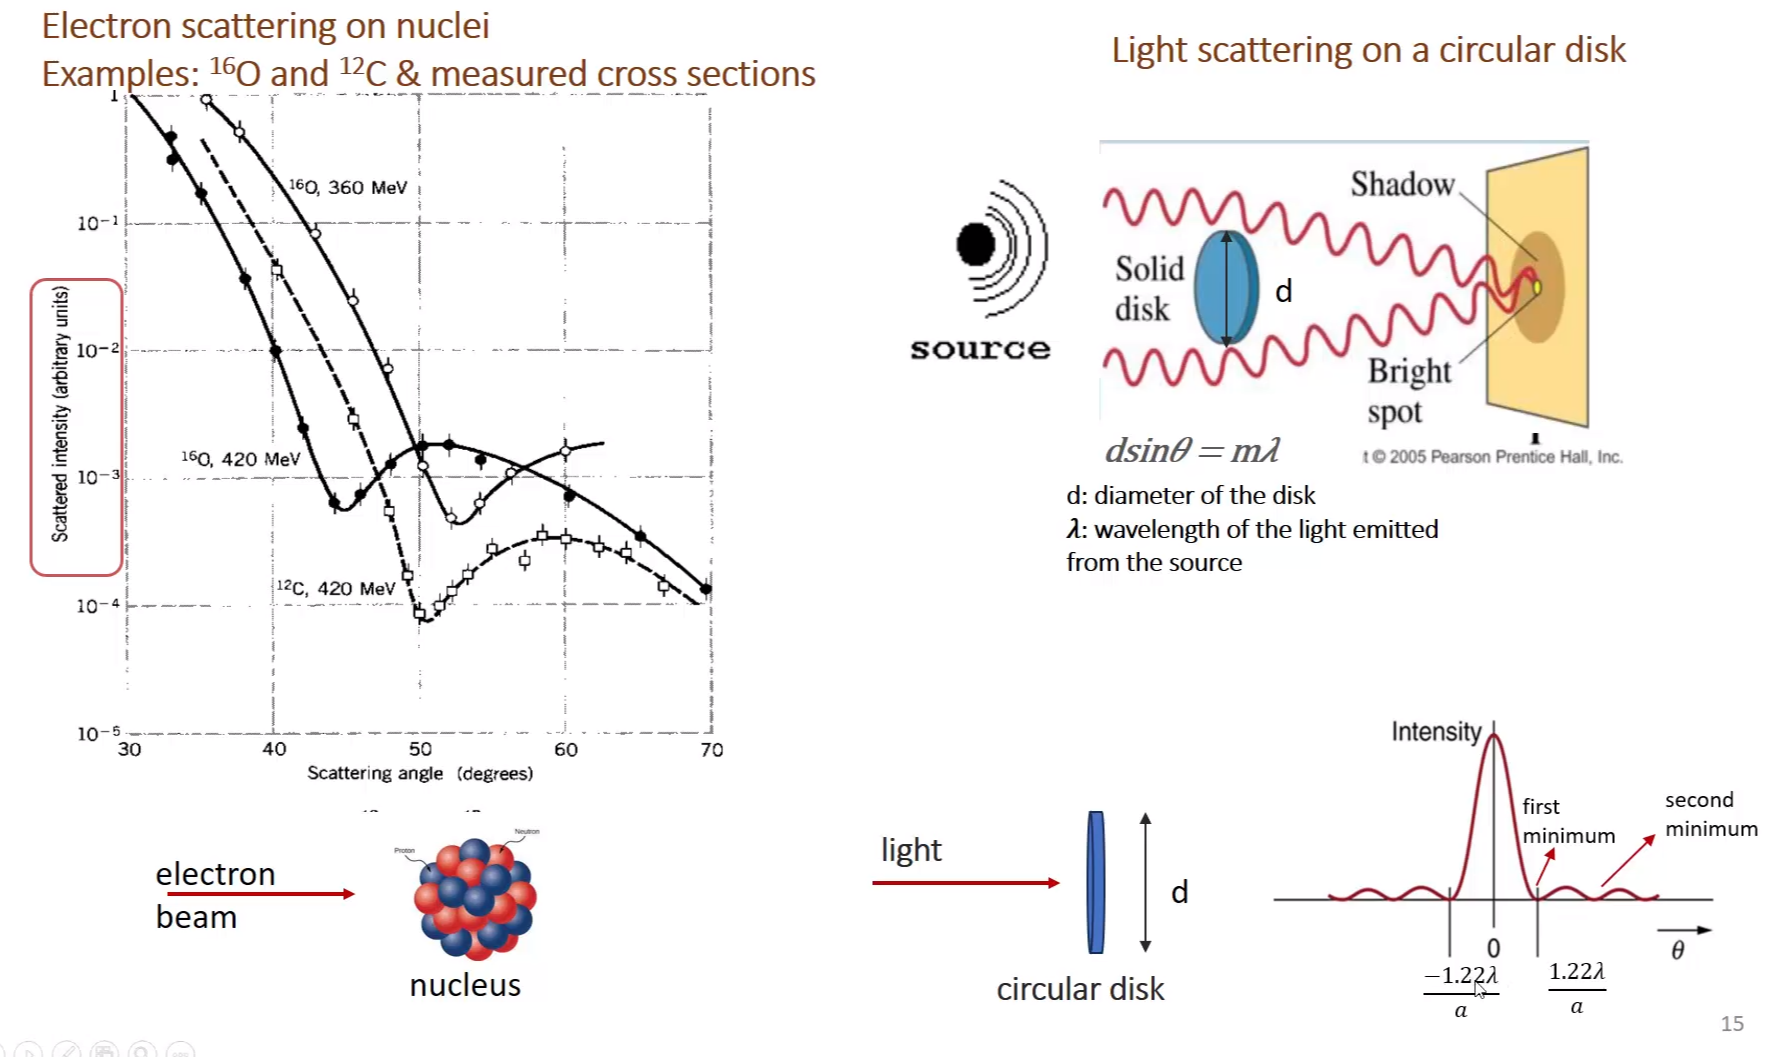
\includegraphics[width = \textwidth]{electron_scattering_angles.png}
\caption{Example of the local minimum of the Rutherford cross-section. The angle is used to calculate the radius of the nucleus.}
\label{fig: electron_scattering_angles}
\end{figure}
\begin{equation}
\sin θ = \frac{1.22λ}{d} ⇒ R = \frac{d}{2} = \frac{1.22λ}{2\sin θ}
\end{equation}
This is only a rough estimate as the angle is calculated in two dimensions, instead of three. 


\subsection{Nuclear Mass Distribution from Hadron Scattering}\label{subsec: Nuclear Mass Distribution from Hadron Scattering}
\begin{itemize}
    \item Electrons only mostly interact with protons. We therefore use hadrons to study the mass distribution of the nucleus.
    \item The radius is proportional to the nuclear rather than the Coulomb force. 
    \item The Rutherford experiment showed that the nucleus is a point-like object.
\end{itemize}

\subsubsection{Fixed Angle of Observation with Changing Energy}
\begin{itemize}
    \item At low energies the alpha particles and the $^{208}$Pb nucleus interact with the Coulomb interacting as with Rutherford scattering.
    \item With increasing energy, the repulsion from the Coulomb force is overcome, and the strong force becomes the dominant force. The Rutherford formula no longer holds. 
    \item The alpha particles became absorbed by the nucleus and only a small fraction is scattered. 
    \item When energy is high enough, we get the diffraction pattern.
\end{itemize}

\subsection{Conclusion from Charge Radius Experiments}
\begin{itemize}
    \item The charge and mass radii of nuclei is nearly equal to within about $0.1$fm. 
    \item Both show the same $A^{1/3}$ dependence with $R_0 = 1.2$fm. 
    \item As heavy nuclei have about 50 \% more neutrons than protons, we might expect the neutron distribution to be more extended than the proton distribution. This is not the case as the neutrons pulls inwards, and the protons push outwards, until they are mixed such that the radius is the same. 
\end{itemize}



\subsection{Nuclear Mass}
\subsection{Deflection Spectrometer}
\begin{figure}[ht!]
\centering
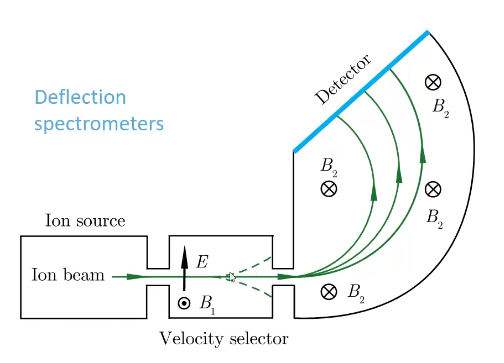
\includegraphics[width = .5\textwidth]{deflection_spectrometer.png}
\caption{Experimental setup for measuring the mass of a particle.}
\label{fig: deflection_spectrometer}
\end{figure}

\begin{itemize}
    \item Shooting a ray of charge particles affected by a magnetic field and measuring the deflection we can calculate its mass. 
    \item To measure an entire particle they must be ionized. The electrons carry so little mass that they are neglected.
    \item After ionization, the particles travel through an electric and magnetic field. 
    \item Only the particles with the right velocity will pass through the fields and be subjected to the new magnetic field. 
    \item The new field will deflect the particles according to their $m / q$ value. 
\end{itemize}
\subsubsection{Calculating the Mass}
\begin{equation}
F_{B} = q \vec{v} × \vec{B} 
\end{equation}
The field and velocity are perpendicular.
\begin{equation}
F_{B} = qvB
\end{equation}
\begin{equation}
F_E = F_B ⇒ qE = qvB ⇒ v = \frac{E}{B_1}
\end{equation}
$B_1$ is the first magnetic field as seen in \cref{fig: deflection_spectrometer}. The force from the magnetic field centripetal force. 
\begin{equation}
F_B = \frac{mv^2}{r} = qvB_2
\end{equation}
\begin{equation}
\frac{mv}{r} = qB_2
\end{equation}
\begin{equation}  
\frac{m}{q} = \frac{B_2ρ}{v}
\end{equation}
The radius of the circle is given by $r = ρ$. Setting $B_1 = B_2$ gives the following for the mass.
\begin{equation}
m = \frac{B_1 B_2 ρ}{E} = \frac{B^2 ρq}{E}
\end{equation}
where $q$ is the charge of the particle.

\paragraph{Accuracy}
\begin{itemize}
    \item These measurements are very important for mass models used in other parts of physics. 
    \item The accuracy is about $Δm / m = 10^{6-}$, but that is not enough. 
    \item The mass doublet technique gives a precision of $10^{-8}$ / $10^{-9}$
\end{itemize}






